\chapter{Entropy of random variables}

Let's reason on the probability of a message. You can consider an infinite sequence of random variables $X_i$ which take values in $\msgset$. We implicitly assumed that $X_i$ are independent random variables. If we group random variables before encoding we can asymptotically reach entropy.

\section{Joint Entropy, Conditional Etropy and Mutual Information}

Given a random variable $X$, the entropy of $X$ is defined as $$H(X) = H(P_X),$$ where $P_X$ is the distribution of $X$. How is entropy defined for two random variables? If $X=Y$ then $H(X, Y) = H(X).$

\begin{definition}[Joint Entropy]
In general, the entropy of a pair is the entropy of the random variable derived by the pair, \emph{i.e.}
\begin{equation}
H(X, Y) = H((X, Y)), 
\end{equation}
since $(X, Y)$ has a probability distribution $P_{XY}$ and we can think of the pair as just a random variable. $H(X, Y)$ is defined a the \emph{joint entropy} of $X$ and $Y$. 
\end{definition}



\begin{prop}
 $$H(P) \leq log(|\xset|),$$ with $P|\xset$ and with equality iff $P(x) = \ifrac{1}{|\xset|}, \forall x \in \xset.$
\end{prop}
\noindent\textbf{Proof}. Call $U$ the uniform distribution. $D(P||U)\geq 0$, with equality iff $P = U$.

\begin{align*}
 D(P||U) & = \sum_{x \in \xset} P(x)\log\left(\dfrac{P(x)}{\sfrac{1}{|\xset|}}\right)\\
 & = \sum_{x \in \xset} P(x)\log(x) + \sum_{x\in\xset} P(x)\log(|\xset|)\\
 & = -H(P) + \log(|\xset|).
\end{align*}

this quantity is nonnegative with equality to zero iff $P=U.$\\

$\hfill\Box$

We write $X \in \xset$ since $X$ is like an unknown element of $\xset$. Random variables don't always have an expected value. We can think of $H(X)$ as the information content of $X$. If we consider entropy as the amount of information in a random variable, then it should be that $H(X, Y) \geq X$. We can think of entropy as  measure over a set.

\[
 H(X) \sim \mu(A),\ A \subseteq U
\]
\[
H(X, Y) \sim \mu(A \cup B),\ \mu(A \cup B) \geq \mu(A)
\]

\begin{prop}
  $$H(X, Y) \geq H(X).$$
\end{prop}

\noindent\textbf{Proof}. Consider the following quantities.

\[ 
H(X, Y) = \sum_{x\in \xset} \sum_{y \in \yset} Pr\{X=x, Y=y\}\log\left(\dfrac{1}{Pr\{X=x, Y=y\}}\right)
\]
and
\begin{align*}
 H(X) &= \sum_{x\in \xset}Pr\{X=x\}\log\left(\dfrac{1}{Pr\{X=x\}}\right)\\
 &=\sum_{x\in\xset}\sum_{y\in\yset}Pr\{X=x, Y=y\}\log\left(\dfrac{1}{Pr\{X=x\}}\right) 
\end{align*}

We take the difference between the two:

\[
 H(X, Y) - H(X) =  \sum_{x\in\xset}\sum_{y\in\yset}Pr\{X=x, Y=y\}\log\left(\dfrac{Pr\{X=x\}}{Pr\{X=x, Y=y\}}\right).
\]

We can think of $Pr\{X=x, Y=y\} = Pr\{X=x\}Pr\{Y=y | X=x\}$, then

\[
  \sum_{x\in \xset} \sum_{y \in \yset} Pr\{X=x\}Pr\{Y=y | X=x\}\log\left(\dfrac{1}{Pr\{Y=y|X=x\}}\right) =
\]
\[
 \sum_{x\in \xset}Pr\{X=x\}\sum_{y \in \yset} Pr\{Y=y | X=x\}\log\left(\dfrac{1}{Pr\{Y=y|X=x\}}\right).
\]

We would like to say that this quantity is nonnegative. Since $H(\cdot)$ is nonnegative, this difference is actually greater than (or equal to) zero.

\begin{definition}[Conditional Entropy]
We call
\begin{equation}
 H(Y|X) = H(X, Y) - H(X)
\end{equation}
the \emph{conditional entropy} of $Y$ given $X$.

\end{definition}


$H(X, Y) - H(X)$ is the convex combination of the entropies of the conditional distribution of $Y$ given the various values of $X$. It's like the expected value of the entropy of the conditional distribution $Pr\{Y=y | X=x\}$.

It can be seen as the residual information when $X$ is known.

\begin{prop}
\begin{equation}
H(Y) \geq H(Y|X). 
\end{equation}
\end{prop}

\noindent\textbf{Proof}. 
\begin{align*}
 H(Y) - H(Y|X) & = \sum_{x \in \xset} \sum_{y \in \yset}Pr\{X=x, Y=y\}\log\left(\dfrac{1}{Pr\{Y=y\}}\right)\\ 
 & - \sum_{x \in \xset}\sum_{y \in \yset} Pr\{X=x, Y=y\}\log\left(\dfrac{Pr\{X=x\}}{Pr\{X=x, Y=y\}}\right)\\
  & =  \sum_{x\in \xset} \sum_{y \in \yset} Pr\{X=x, Y=y\}\log\left(\dfrac{Pr\{X=x, Y=y\}}{Pr\{X=x\}Pr\{Y=y\}}\right). 
\end{align*}



This is symmetrical in $X$ and $Y$. Notice that $H(Y) - H(Y|X)$ is not. This also looks as a log sum inequality. In Particular, it is similar to information divergence of the distribution $P_{XY}$ from the distribution $P_X \times P_Y$. So,

\begin{equation}
 H(Y) - H(Y|X) = D(P_{XY}||P_X \times P_Y) \geq 0 
\end{equation}


and we have equality when $P_{XY} = P_X \times P_Y$. It is a measure of indipendence of $X$ and $Y. \hfill\Box$
\begin{definition}[Mutual Information]
We define the amount of information that $X$ and $Y$ share as follows:
\begin{equation}
I(X \wedge Y) = H(Y) - H(Y|X), 
\end{equation}
and it is called mutual information. It is symmetric and nonnegative. 
\end{definition}

Notice that
\begin{align*}
 I(X \wedge Y) &= H(Y) - H(Y|X) \\&= H(Y) + H(X) - H(X, Y) 
\end{align*}
thus
\begin{equation}
 H(X, Y) \leq H(X) + H(Y) 
\end{equation}

with equality iff $X$ and $Y$ are independent. Finally, we state (without proof) that
\begin{equation}
 H(Y|Z) \geq H(Y |Z, X). 
\end{equation}

\begin{prop}[Chain Rule]
The \emph{chain rule} states that
\begin{equation}
 H(X_1, \ldots, X_n) = H(X_1) + \sum_{i = 2}^n H(X_i | X_1, \ldots, X_{i-1}).
\end{equation}
\end{prop}

We have said that $I(X \wedge Y) \sim \mu(A \cap B)$, and since $H(Y | X, Z) \leq H(Y|Z)$ we can state that

\[
 I(X\wedge Y | Z) \sim \mu(A \cap B \setminus C)
\]

that is the conditional mutual information. We now wonder about which quantity between $I(X \wedge Y | Z)$ and $I(X \wedge Y)$ is greater.

\begin{align*}
 I(X \wedge Y) -  I(X\wedge Y | Z)  & \sim \mu(A \cap B) - \mu((A \cap B) \setminus C)\\
 & = \mu((A \cap B) \setminus ((A \cap B) \setminus C)) \\ 
 & = \mu(A \cap B \cap C). 
\end{align*}

this is what the analogy suggests, but we need a proof to believe that this is true.

\begin{equation}\label{eq:mutcondinf}
 I(X \wedge Y) - I(X \wedge Y | Z) \geq 0
\end{equation}

If $X \equiv Y \equiv Z$ then
\begin{equation}
I(X \wedge X) = H(X) - H(X|X) = H(X) 
\end{equation}

so Equation \ref{eq:mutcondinf} is possible. We can also have it the other way around:
\begin{equation}
I(X \wedge Y | Z) \geq I(X \wedge Y). 
\end{equation}

It follows that equality does not hold. Suppose $X, Y, Z \in \{0, 1\}$, and also they are uniformly distributed. Moreover, $X$ and $Y$ are independent so $I(X \wedge Y) = 0$. We then define $Z = X \oplus Y$, but then $X = Y \oplus Z$ and $Y = X \oplus Z$. $X, Y, Z$ are pairwise independent, but they are not three-way independent, since every couple of them determines the third.

\[
 I(X\wedge Y|Z) = H(X|Z) - H(X|Y, Z) = H(X) - 0 = 1.
\]

Any number $m \geq 2$ of sets are disjoint iff they are pairwise disjoint, but random variable independence does not satisfy this property. The analogy fails on assuming that random variables independence is similar to set disjointness. $n$-way independence is binary, but $n$-way independence is unrelated to $m$-way independence if $n \not= m$.

\section{Information Source and Speed of Information}

An \emph{information source} is an infinite sequence $X_1, X_2, \ldots, X_n$ of random variables with $X_i \in \xset$, \emph{i.e.} they take values from the same set. How can we measure the information content in an information source? We denote the information source as $X^\infty$, commonly $X^n = X_1, \ldots, X_n$. 

The ``speed'' of information from a sequence of random variables is $$\dfrac{1}{n}H(X_1, \ldots, X_n).$$
The information rate of $H^\infty$, if it exists, is

\[
 \lim_{n \rightarrow \infty} \dfrac{1}{n}H(X^n).
\]

Consider $\{X_i\}_{i = 1}^\infty$, i.i.d., and denote by $P$ the common distribution of $\{X_i\}_{i = 1}^\infty$, so that $H(X_i) = H(P),\ \forall i.$

In this case,

\[
 H(X_1, \ldots, X_n) = \sum_{i = 1}^n H(X_i) = nH(P)
\]

so
\[
 \lim_{n \rightarrow \infty} \dfrac{1}{n}H(X^n) = H(P).
\]

What is the sufficient condition for this to hold (i.e. for the limit to exists)? We need stationary random variables: impredictable but ``stationary''. We call an information source $\{X_i\}_{i = 1}^\infty$ \emph{stationary} if 
\[
 \forall n,k \in \mathbb{N},\ \forall \str{x} \in \xset^n\ Pr\{X^n=\str{x}\} = Pr\{X_{k+1}, \ldots, X_{k+n} = \str{x}\}.
\]

We will see that if an information source is stationary then it has an information rate. In particular, with a stationary source the sequence $$H(X_i | X_1, \ldots, X_{i-1})$$ decreases.

We call an information source \emph{memoryless} if $X_i, \forall i$, are totally independent. We will show that lack of memory is not a sufficient condition for the existence of the information rate.

Consider $\{X_i\}_{i = 1}^\infty$, a sequence of totally independent random variables, does its entropy rate exists?

\[
 \dfrac{1}{n}H(X_1, \ldots, X_n) = \dfrac{1}{n}\left(\sum_{i=1}^nH(X_i)\right)
\]
when does this quantity diverge. Take $H(X_i) \in \{0, 1\}$, the question is
\[ 
\exists? \lim_{n\rightarrow \infty} \sum_{i = 1}^n \dfrac{\epsilon_i}{n},\ \epsilon_i \in \{0, 1\}
\]

\begin{figure}[h!]
\centering
	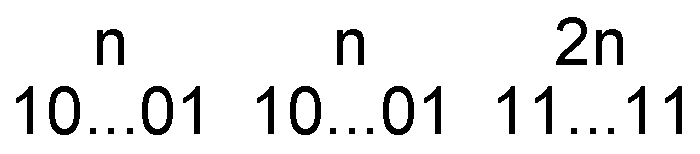
\includegraphics[width=0.3\linewidth]{pictures/ch05-seq.eps}
\end{figure}
the first $2n$ bits, a sequence of alternating bits, have average $\ifrac{1}{2}$. Add the second $2n$ and you get $\ifrac{2}{4}$. Repeat this and the sequence oscillates between $\ifrac{3}{4}$ and $\ifrac{1}{2}$.

\begin{thm}
 If $\{X_i\}_{i = 1}^\infty$ is stationary, then its entropy rate exists.
\end{thm}

\noindent\textbf{Proof}. It's reasonable to think that $$\dfrac{1}{n}H(X_1, \ldots, X_n)$$ goes to 0. It's sufficient to prove this to show that the rate exists (and it's 0). We just show it's decreasing:
\[
 \dfrac{1}{n}H(X_1, \ldots, X_n)  \leq \dfrac{1}{n-1}H(X_1, \ldots, X_{n-1}) 
\]

\emph{i.e.} we prove

\[
 (n-1)H(X^n)  \leq nH(X^{n-1}) 
\]

\[
 (n-1)[H(X^{n-1}) + H(X_n | X^{n-1})]  \leq nH(X^{n-1}) 
\]

we thus have to prove that

\[
  (n-1)H(X_n | X^{n-1})  \leq H(X^{n-1}) 
\]

we apply the definition of joint entropy

\[
 (n-1)H(X_n | X^{n-1})  \leq H(X_1) + \sum_{i=2}^{n-1}H(X_i|X^{i-1}) 
\]

since the source is stationary, we rewrite the right hand side in

\[
 H(X_n) + \sum_{i=2}^{n-1} H(X_n|X_{1 + n - i} \ldots X_{n-1})
\]

the proof then is

\[
(n-1)H(X_n|X^{n-1}) \leq H(X_n) + \sum_{i=2}^{n-1}H(X_n | X_{1+n-i} \ldots X_{n-1}) 
\]

this means something like

\[
 H(X_n|X^{n-1}) \leq H(X_n)
\]
\[
 \vdots
\]

\[
 H(X_n|X^{n-1}) \leq H(X_n | X_{1+n-i} \ldots X_{n-1}) 
\]
\[
 \vdots
\]
\[
 H(X_n|X^{n-1}) \leq H(X_n|X^{n-1})
\]

for $n+1$ times for $i \in [2, n-1]$. Look at the generic term

\[
 H(X_n|X_1 \ldots X_{n-1}) \leq H(X_n|X_{n-k}\ldots X_{n-1}),\ \forall k
\]

this is

\[
 H(X_n | X_{n-k} \ldots X_{n-1}) -H(X_n|X_1\ldots X_{n-1}) =
\]
\[
 I(X_n \wedge X_1 \ldots X_{n-k-1} | X_{n-k} \ldots X_{n-1}) \geq 0
\]
that remind us

\[
 I(A \cap B | C) \geq 0 \Rightarrow H(A|C) \geq H(A | B,C).
\]
$ \hfill\Box$

\section{Universal compression}
Lempel and Ziv worked on universal compression algorithms. Universal compression is possible with stationary source. How would you compress a stationary source to its entropy?

Consider $\{X_i\}_{i=1}^\infty$, that is stationary. Given $f$, a variable length prefix code, we consider $|f(X_i)|$ as a random variable. We can talk about the expected value $E|f(X_i)|$. We know that
\[
 H(X_i) \leq E|f(X_i)| \leq H(X_i) + 1
\]
now,
\[
|f(X_1)\ldots f(X_n)| = \sum_{i=1}^n|f(X_i)|. 
\]

\[
 \dfrac{1}{n}\sum_{i=1}^n H(X_i) \leq\dfrac{1}{n}\sum_{i=1}^n |f(X_i)|
\]

if the source is stationary all variables have distribution $P$.
\[
 H(P) \leq \dfrac{1}{n} \sum_{i = 1}^n |f(X_i)| \leq H(P) + 1
\]
but we didn't get far. Instead, join random variables together. Let $f_n$ be an optiman (in the sense of length of output) prefix code for $X_1 \ldots X_n$.
\[
 \dfrac{1}{k}H(X^k) \leq \dfrac{1}{k}E(|f_n(X^k)|) \leq \dfrac{1}{k}[H(X^k) + 1]
\]

if $k \rightarrow \infty$ (and we enlarge the conding window), both sides go to the entropy rate. Thus the entropy is the ``limit''.
